% Experiment

\chapter{Experimental Setup}
\label{ch:experimental-setup}

For the experimentation phase we have used a Intel Core i7-6700HQ CPU
@ 2.60GHz, with 16GB of RAM, and a Cuda enabled Nvidia GeForce GTX
960M graphic card.

The data-set previously described in \autoref{part:variables} has been
pre-processed. This process consisted in narrowing down the data to
the same date range. Later the missing values where filled with
interpolated values. Finally the data-set has been normalized using a
standard score described in \autoref{eq:standard-score}.

\begin{equation}
  \begin{aligned}
    \label{eq:standard-score} X_{norm} & = \frac{X-\mu}{\sigma} \\
X_{norm} & \leftarrow \text{Normalized instance} \\ X & \leftarrow
\text{Original instance} \\ \mu & \leftarrow \text{Feature mean} \\
\sigma & \leftarrow \text{Feature standard deviation} \\
  \end{aligned}
\end{equation}

After predicting the values of the BTC price, the values are still
normalized. In order to correctly interpret them and compute the error
measures, this prediction has been de-normalized using the inverse
function of \autoref{eq:standard-score}, which is represented in
\autoref{eq:inverse-standard-score}.

\begin{equation}
  \begin{aligned}
    \label{eq:inverse-standard-score} \hat{X} & = \hat{X}_{norm}
\times \sigma + \mu \\ \hat{X}_{norm} & \leftarrow \text{Normalized
prediction} \\ \hat{X} & \leftarrow \text{De-normalized prediction} \\
\mu & \leftarrow \text{Feature mean} \\ \sigma & \leftarrow
\text{Feature standard deviation} \\
  \end{aligned}
\end{equation}

The layout of the network is the \textit{fully connected recurrent
neural network} which is shown in \autoref{fig:rnn-topology}.

\begin{figure}[bth] \myfloatalign
{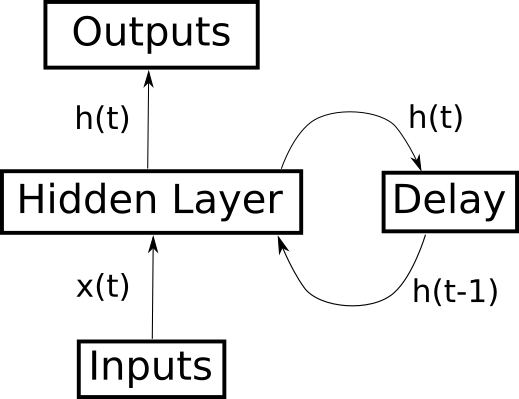
\includegraphics[width=.4\linewidth] {gfx/rnn-topology}}
  \caption{\textit{RNN} topology.}
  \label{fig:rnn-topology}
\end{figure}

The first layer is composed of 1 neuron per instance, the hidden layer
is composed of another neuron per instances, and the output is
composed of only one neuron. More details related to \textit{RNNs} can
be found in \autoref{part:method-technique}.

After the pre-processing, and to avoid over-fitting we have used
\textit{time series cross-validation} proposed by
\cite{robjhyndman2010}. The particular implementation of this
technique used uses a test partition of size 1, which we call $x_{t +
1}$ and a train partition composed of all the elements from the
$1095$-th to the $t$-th. The details about why we used $1095$-th as
the first element and the overall technique can be found in
\autoref{part:implementation}.

\chapter{Experimental Results}
\label{ch:experimental-results}

\section{Results introduction}
\label{sec:result-presentation}

In this section we present the results of the experiments performed.
We decided that we would compare the performance of \textit{RNN} with
a traditional method such as \textit{VAR}.

Both \autoref{fig:predictions-subplots} and \autoref{fig:predictions}
represent a day ahead prediction of the Bitcoin price, compared to the
actual Bitcoin price, shown in the variable \textit{MarketPrice}. It
is the same information presented in two different ways to allow the
viewer to see the particular values of each one in
\autoref{fig:predictions-subplots}, and, on the other side, to be able
to compare closely the values of the two models and
\textit{MarketPrice} in \autoref{fig:predictions}.

\begin{figure}[bth] \myfloatalign {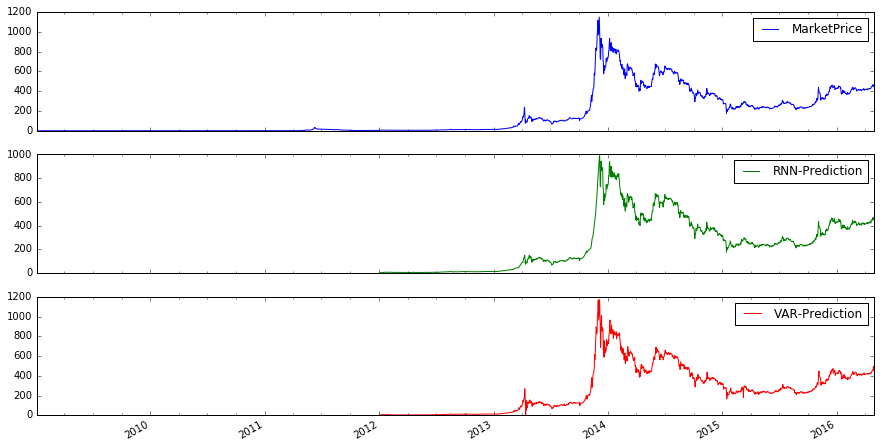
\includegraphics[width=1\linewidth]
{gfx/predictions-subplots}}
  \caption{Predictions models and \textit{MarketPrice} true values in
separate charts.}
  \label{fig:predictions-subplots}
\end{figure}

Although the shapes of the charts are similar, it can be noticed how
\textit{RNN} takes more instances to learn certain patterns, like the
one present in the first quarter of 2013, where \textit{RNN} doesn't
have the spike that \textit{VAR} and \textit{MarketPrice} do have.
This behavior is better perceived in the upper-right chart of
\autoref{fig:predictions}.

\begin{figure}[bth]
  \myfloatalign {
    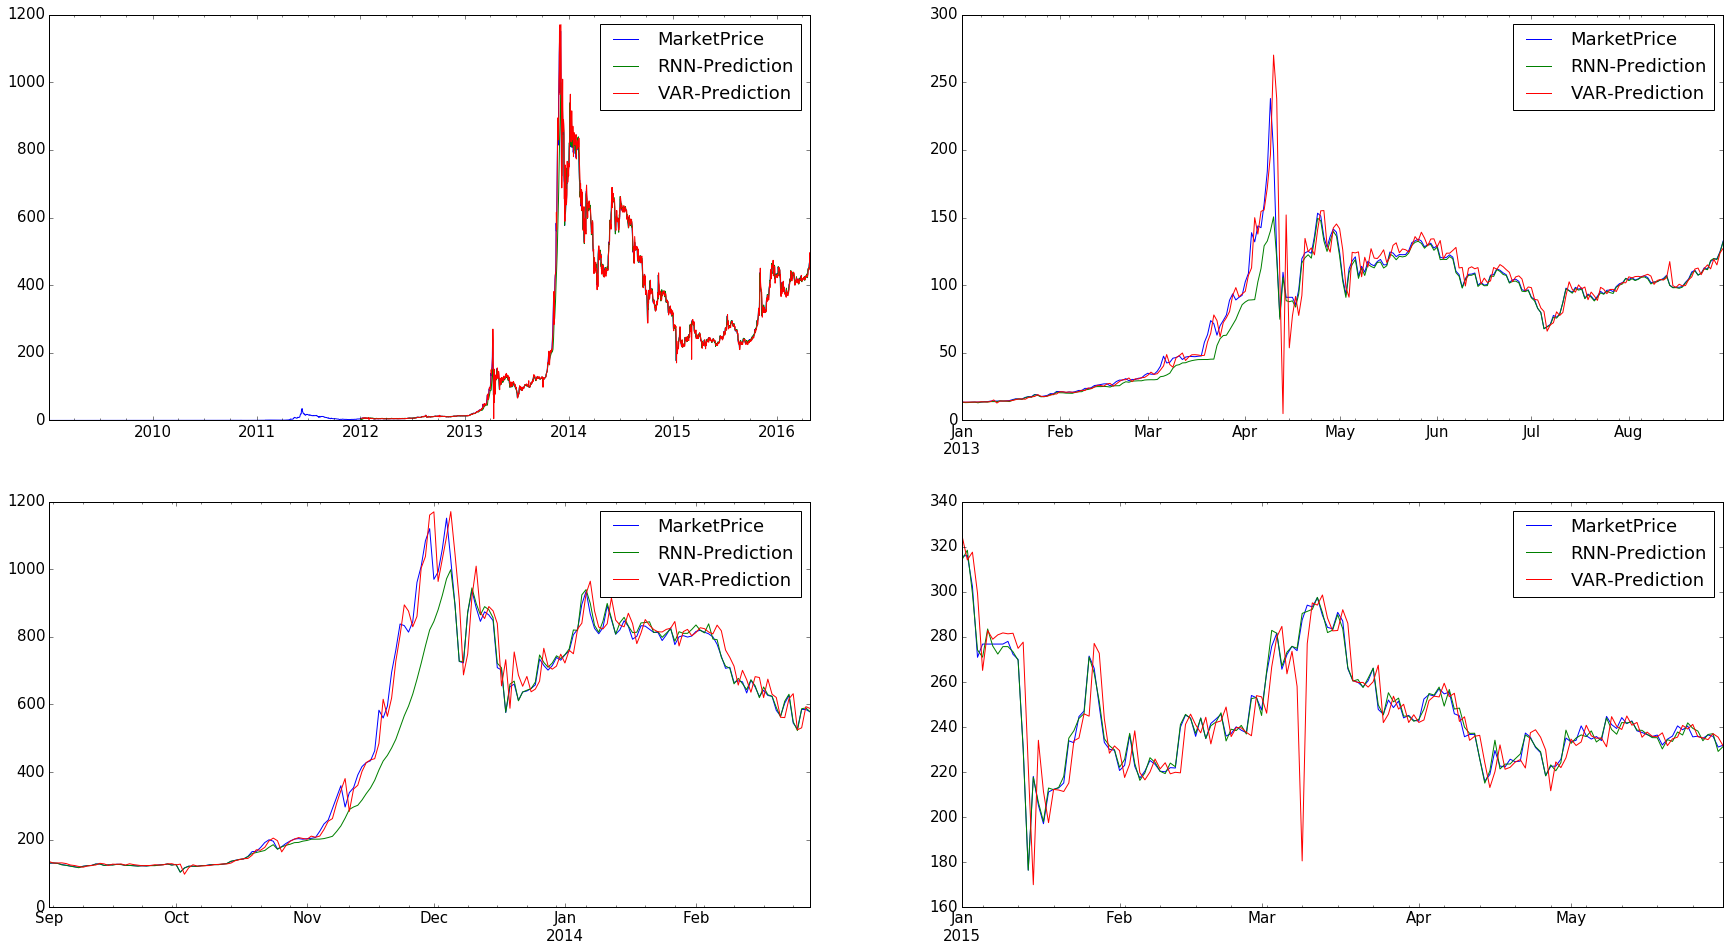
\includegraphics[width=1\linewidth]
    {gfx/predictions}}
  \caption{Prediction models and \textit{MarketPrice} true values in
    the same chart.}
  \label{fig:predictions}
\end{figure}

\textit{RNN} has a tendency to have lower values than those of
\textit{VAR} and \textit{MarketPrice}. When the change in the price is
high \textit{RNN} doesn't change at the same pace while \textit{VAR}
follows the tendency better. On the other hand, when the \textit{BTC}
price decreases, there are some times that \textit{VAR} makes a big
descent after \textit{MarketPrice} decreases. It can be observed in
the upper-right and lower-right charts of \autoref{fig:predictions}.

\section{Accuracy measures}
\label{sec:accuracy-measures}

The main accuracy measure used is \textit{mean absolute error (MAE)},
shown in \autoref{eq:mae-expression}, averages the absolute error
produced for every prediction done with a particular model. This error
measure has the characteristic of represent quantities in the same
unit as the original variable and that is easily understandable.

When the fluctuation of the \textit{BTC} price are low, \textit{RNN}
is closer to \textit{MarketPrice} than \textit{VAR}, which can be seen
in \autoref{fig:comparison-histogram-prediction-errors}.

\begin{equation}
  \begin{aligned}
    \label{eq:mae-expression}
    \textit{Mean Absolute Error: MAE} & =
    \frac{1}{n} \sum_{i=1}^{i=n} |e_i|\\
    e_i & = y_i - \hat{y}_i
  \end{aligned}
\end{equation}

In \autoref{tab:forecast-accuracy-measures} we present another error
measures to compare the predictions made by \textit{VAR} and
\textit{RNN}. The next accuracy measure to \textit{MAE} is
\textit{mean squared error (MSE)}, shown in
\autoref{eq:mse-expression}, which doesn't present the prediction
errors in the same unit, but has the feature of giving more importance
to bigger errors, than smaller ones. To see how this two measures
gives us different information about the same data we can see in
\autoref{tab:forecast-accuracy-measures} that, while \textit{RNN}'s
\textit{MAE} is lower than \textit{VAR}'s \textit{MAE}, the
\textit{RNN}'s \textit{MSE} is bigger than \textit{VAR}'s. That is
because \textit{RNN} errors are bigger and at the same time it has
less small errors. That can be clearly seen in
\autoref{fig:comparison-histogram-prediction-errors}.

\begin{figure}[bth]
  \myfloatalign {
    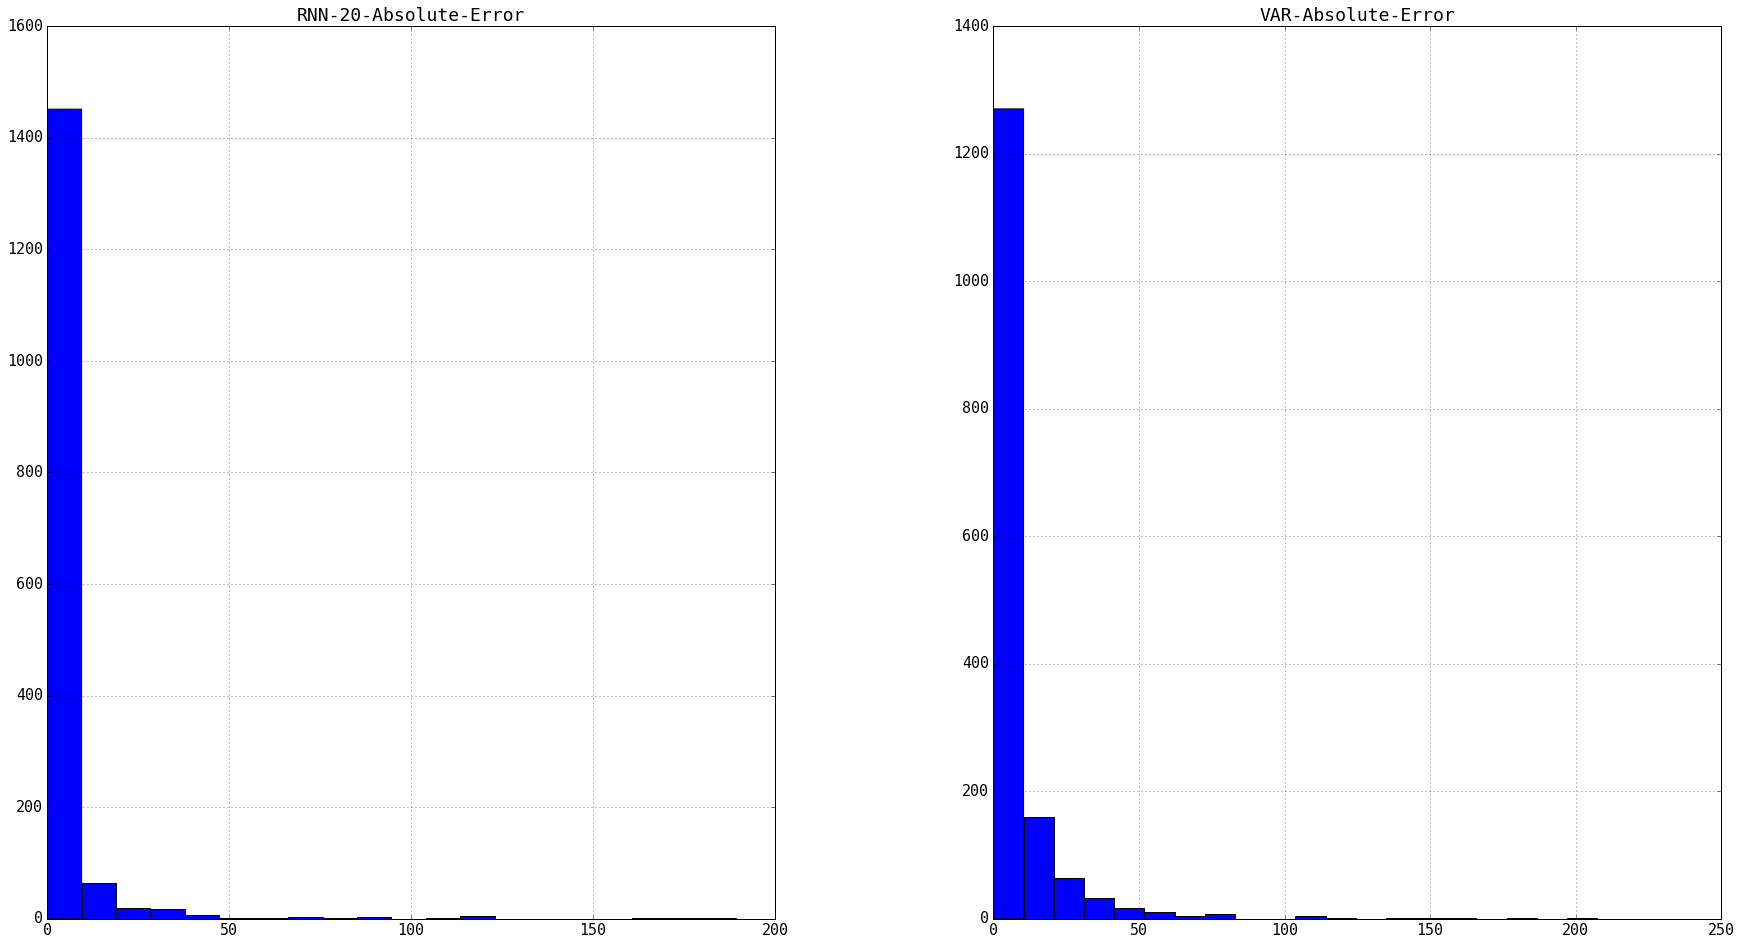
\includegraphics[width=1\linewidth]
    {gfx/comparison-histogram-prediction-errors}}
  \caption{Histogram of \textit{RNN} absolute errors and \textit{VAR}
    absolute errors.}
  \label{fig:comparison-histogram-prediction-errors}
\end{figure}

\begin{equation}
  \begin{aligned}
    \label{eq:mse-expression}
    \textit{Mean Squared Error: MSE} & = \frac{1}{n} \sum_{i=1}^{i=n} e_i^2\\
    e_i & = y_i - \hat{y}_i
  \end{aligned}
\end{equation}

\begin{table}[bth]
  \myfloatalign
  \small
  \begin{tabularx}{\textwidth}{Xcc}
    \toprule \tableheadline{Measure Type} &
    \tableheadline{RNN Value}
    & \tableheadline{VAR Value} \\
    \midrule
    \textit{Mean absolute error (MAE)} & $5.4$ & $8.57$ \\
    \textit{Mean squared error (MSE)} & $638.55$ & $367.82$ \\
    \textit{Mean absolute percentage error (MAPE)} & $3.19$ & $3.46$ \\
    \textit{Theil's U statistic} & $0.47$ & $0.03$ \\
    \bottomrule
  \end{tabularx}
  \caption{Forecast accuracy measures}
  \label{tab:forecast-accuracy-measures}
\end{table}

Another accuracy measure used is \textit{mean absolute percentage
  error (MAPE)}, defined in \autoref{eq:mape-expression}. This measure
is useful when there are several scales, for example if the models are
run over different data-sets. This measure have the disadvantage of
being undefined for $y_i = 0$, and that it puts a heavier penalty on
negative errors than on positive errors.

\begin{equation}
  \begin{aligned}
    \label{eq:mape-expression}
    \textit{Mean Absolute Percentage Error: MAPE} & = \frac{1}{n}
    \sum_{i=1}^{i=n} \frac{100 \times e_i}{y_i} \\
    e_i & = y_i - \hat{y}_i
  \end{aligned}
\end{equation}

Finally we \textit{Theil's U statistic} which is defined in
\autoref{eq:theils-u-statistic}. This measure compares a forecast
model to the actual model. Is the ratio of the 1-step-ahead
\textit{MSE} for a given forecast relative to that of a random walk
forecast. If \textit{Theil's U statistic} is less than 1 then the
forecasting technique is better than guessing, if is exactly 1 then is
about as good as guessing and if it is more than 1 the forecasting
technique is worse than guessing.

\begin{equation}
  \begin{aligned}
    \label{eq:theils-u-statistic}
    \textit{Theil's U statistic} & = \sqrt{\frac {\displaystyle\sum_{t
          = 1}^{n - 1} \left( \frac{\hat{y}_{t+1} - y_{t+1}}{y_t}
        \right)^2} {\displaystyle\sum_{t = 1}^{n - 1} \left(
          \frac{y_{t+1} - y_t}{y_t} \right)^2}}
  \end{aligned}
\end{equation}

We can see in \autoref{tab:forecast-accuracy-measures} that the value
of \textit{Theil's U statistic} for \textit{RNN} is greater than that
of \textit{VAR} which can be understood as \textit{RNN} being closer
to $1$, so it's a worse forecasting technique than \textit{VAR} that
is closer to $0$.

\section{Errors analysis}
\label{sec:errors-analysis}

\autoref{fig:comparison-errors} shows an important information to be
able to understand how do the two prediction models studied behave.

\begin{figure}[bth]
  \myfloatalign
  {
    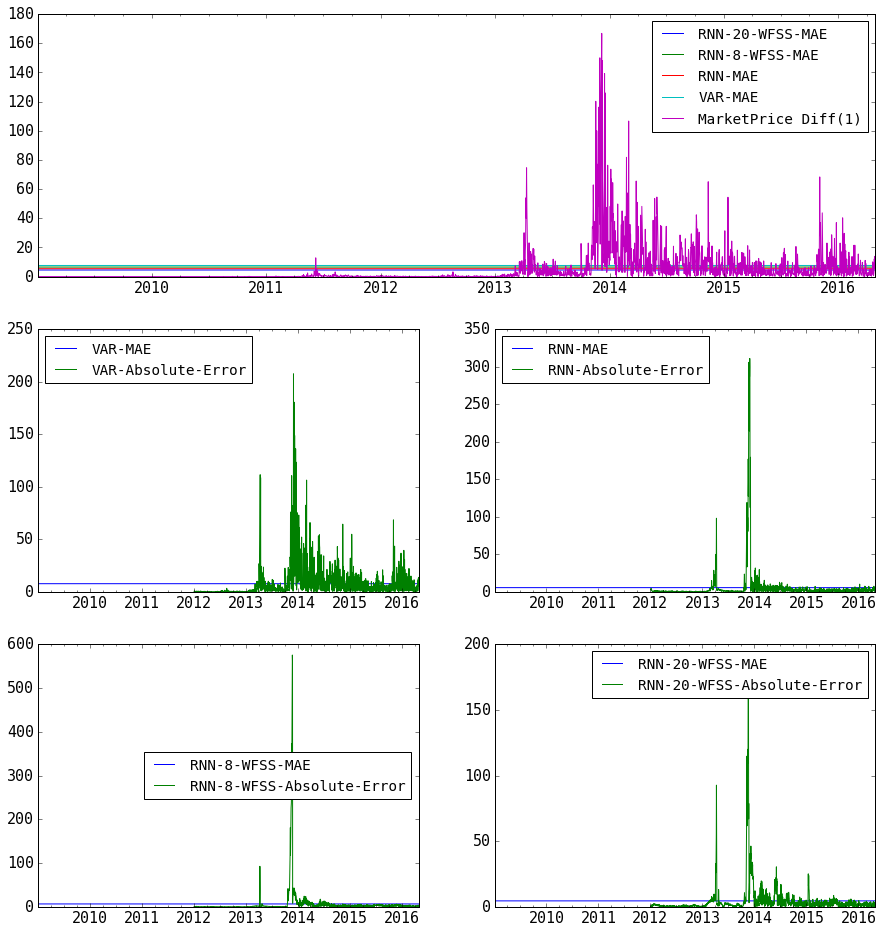
\includegraphics[width=1\linewidth]
    {gfx/comparison-errors}}
  \caption{Error graphs.}
  \label{fig:comparison-errors}
\end{figure}

First off we can see the comparison between the \textit{MAE}'s of each
model and the fluctuation (formally know as first difference or
\textit{Diff(1)}) of the \textit{BTC} price. It's important to note
that for the two models the \textit{MAE} is mostly beneath the daily
fluctuation of \textit{BTC}, which tells us the the error is
relatively small to predict the \textit{MarketPrice}.

In the two lower graphs of \autoref{fig:comparison-errors} we see a
comparison of model's \textit{MAE} and absolute errors. The errors of
\textit{RNN} are located around two events of huge change of the
\textit{MarketPrice}. There the errors of \textit{RNN} are higher than
those of \textit{VAR}. That's the reason why \textit{RNN} as higher
penalties for bigger errors and those higher \textit{MSE} than
\textit{VAR}. On the contrary, in the rest of the time series
the errors of \textit{VAR} exceed those of \textit{RNN}, which is the
reason why \textit{RNN's} \textit{MAE} is lower than \textit{VAR's}.

Regarding the errors probability distribution we would benefit from it
to be normal, because that way we would be able to establish a
confidence interval with the normal distribution parameters with the
expression in \autoref{eq:confidence-interval}.

\begin{equation}
  \begin{aligned}
    \label{eq:confidence-interval}
    \textit{Confidence interval} & =
    [ \hat{x} - 2 \sigma, \hat{x} + 2 \sigma ]
  \end{aligned}
\end{equation}

In \autoref{fig:normal-fitted-to-errors} we can see the shape of the
error's histograms plotted along a fitted normal distribution.
Visually the shape of the normalized histograms resembles that of the
fitted normal distributions but we need more evidence. Hence we've run
several normality tests in order to ensure that the distribution of
the errors can be considered to be normal.

\begin{figure}[bth]
  \myfloatalign
  {
    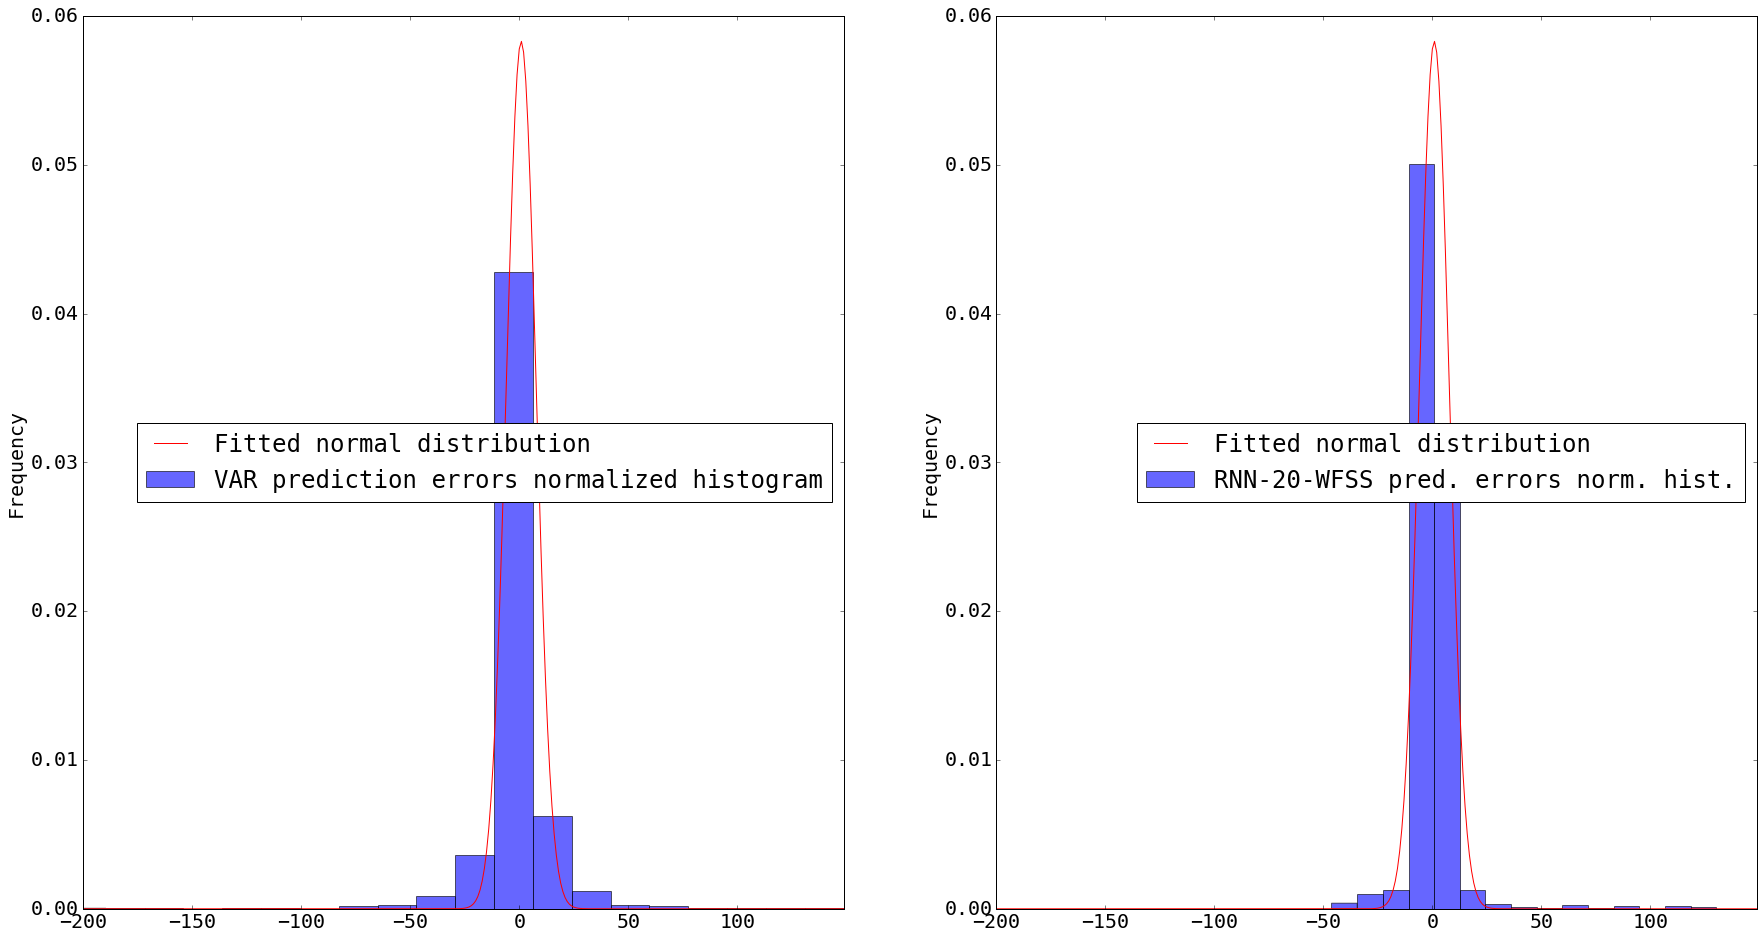
\includegraphics[width=1\linewidth]
    {gfx/normal-fitted-to-errors}}
  \caption{Normal fitted to prediction errors.}
  \label{fig:normal-fitted-to-errors}
\end{figure}

In \autoref{tab:normality-test-results} we can see the results of all
the normality tests performed, namely \textit{skewness test},
\textit{kurtosis test}, and \textit{D’Agostino and Pearson's
  ``omnibus'' test}.

\textbf{Skewness} (\cite{d1970transformation}) - Is a measure of the
asymmetry of the probability distribution of a random variable about
its mean. In other words, skewness tells you the amount and direction
of skew (departure from horizontal symmetry). The skewness value can
be positive or negative, or even undefined. If skewness is $0$, the
data are perfectly symmetrical, although it is quite unlikely for
real-world data. As a general rule of thumb:

\begin{itemize}
\item If skewness is less than -1 or greater than 1, the distribution
  is highly skewed.
\item  If skewness is between -1 and -0.5 or between 0.5
  and 1, the distribution is moderately skewed. 
\item If skewness is between
  -0.5 and 0.5, the distribution is approximately symmetric.
\end{itemize}

The mathematical expression of the skewness measure is defined in
\autoref{eq:skewness-measure}.

\begin{equation}
  \begin{aligned}
    \label{eq:skewness-measure}
    \textit{Skewness Measure} & = \frac{m_3}{m_2^{3/2}}
  \\
  m_k & = \frac{1}{n} \displaystyle\sum_{i=1}^n (x_i - \bar{x} )^k
  \end{aligned}
\end{equation}

\begin{table}[bth]
  \myfloatalign
  \small
  \begin{tabularx}{\textwidth}{Xcc}
    \toprule \tableheadline{Type of test} &
    \tableheadline{Statistic test value}
    & \tableheadline{P-Value} \\
    \midrule
    \textit{VAR Skewness test} & $-23.33$ & $1.85e-120$ \\
    \textit{RNN Skewness test} & $41.34$ & $0.0$ \\
    \textit{VAR Kurtosis test} & $21.33$ & $5.34e-101$ \\
    \textit{RNN Kurtosis test} & $25.09$ & $5.38e-139$ \\
    \textit{VAR D’Agostino and Pearson omnibus test} & $999.81$ & $7.80e-218$ \\
    \textit{RNN D’Agostino and Pearson omnibus test} & $2339.06$ & $0.0$ \\
    \bottomrule
  \end{tabularx}
  \caption{Normality test results}
  \label{tab:normality-test-results}
\end{table}

We can see by the results of the test in
\autoref{tab:normality-test-results} that the distribution of the
errors of the two models are skewed. 

\textbf{Kurtosis} (\cite{anscombe1983distribution}) - This measure is
informative about the tail behavior of a series. Kurtosis tells the
height and sharpness of the central peak, relative to that of a
standard bell curve. The mathematical expression is shown
in \autoref{eq:kurtosis-measure}.

\begin{equation}
  \begin{aligned}
    \label{eq:kurtosis-measure}
    \textit{Kurtosis Measure} & =
    \frac{m_4}{m_2^2} - 3 \\
      m_k & = \frac{1}{n} \displaystyle\sum_{i=1}^n (x_i - \bar{x} )^k
  \end{aligned}
\end{equation}

\textbf{D’Agostino and Pearson omnibus} (\cite{d1971omnibus,
  d1973tests}) - This test is a combination of skewness and kurtosis,
called \textit{``omnibus''} test. The mathematical expression is
\autoref{eq:omnibus-measure}. The distribution of the
\textit{``omnibus''} measure  is approximately a $\chi^2$ distribution
with two degrees of freedom under the null hypothesis that the sample
was drawn from a population with normally distributed values.

\begin{equation}
  \begin{aligned}
    \label{eq:omnibus-measure}
    \textit{Omnibus Measure} & =
    ((\frac{m_3}{m_2^{3/2}})^2 + (\frac{m_4}{m_2^2})^2\\
    m_k & = \frac{1}{n} \displaystyle\sum_{i=1}^n (x_i - \bar{x} )^k
  \end{aligned}
\end{equation}

Given that the null hypothesis is that the samples in the errors set
are drawn from a normal distribution and the p-values are less than
0.01, the aforementioned null hypothesis gets rejected. In light of
this results we can't conclude that the errors are normally
distributed.

%---------------------------------------------------------------------
%---------------------------------------------------------------------
%---------------------------------------------------------------------

%\enlargethispage{2cm}

%------------------------------------------------

%%% Local Variables:
%%% mode: latex
%%% TeX-master: "../main"
%%% End:
